\documentclass[14pt,oneside,a4paper]{extreport}
\usepackage{vntex}
\usepackage{import}
\usepackage{titlesec}
\usepackage{indentfirst}
\usepackage{geometry}
\usepackage{tabularx}
\usepackage{fancyhdr}
\usepackage{tikz}
\usepackage[absolute,overlay]{textpos}
\usetikzlibrary{calc}
\usepackage{graphicx}
\graphicspath{ {./images/} }

\geometry{
	a4paper,
	total={160mm,252mm},
	left=35mm,
	top=25mm,
}

\pagestyle{fancyplain}
\fancyhf{}
\fancyhead[C]{\thepage}
\renewcommand{\headrulewidth}{0pt}

\setlength{\parskip}{10pt}
\titleformat*{\section}{\large\bfseries}
\setlength{\parindent}{2em}

\begin{document}
\tikz[overlay, remember picture]
\draw ($(current page.north west) + (35mm,-25mm)$)
rectangle ($(current page.south east) + (-15mm,20mm)$);

\begin{center}
	
\begin{textblock*}{210mm}(10mm,35mm)
	\large\textbf{HỌC VIỆN KỸ THUẬT QUÂN SỰ}
\end{textblock*}

\end{center}

\begin{textblock*}{210mm}(75mm,70mm)
	\textbf{\normalsize \\
		LÝ VĂN CHẢN \\
		NGUYỄN NGỌC KHÁNH \\
		BÙI ĐÌNH THỦY\\
		KHÓA 15\\
		HỆ ĐÀO TẠO KỸ SƯ DÂN SỰ
	}
\end{textblock*}

\begin{center}

\begin{textblock*}{210mm}(10mm,130mm)
	\textbf{\LARGE ĐỒ ÁN TỐT NGHIỆP ĐẠI HỌC}
\end{textblock*}

\begin{textblock*}{210mm}(10mm,150mm)
	\textbf{CHUYÊN NGÀNH: CÔNG NGHỆ DỮ LIỆU}
\end{textblock*}

\begin{textblock*}{160mm}(35mm,180mm)
	\textbf{\large Đề tài: Nhận diện các phương tiện giao thông đi ngược chiều qua camera lắp đặt cố định tại một tuyến đường}
\end{textblock*}

\begin{textblock*}{210mm}(10mm,260mm)
	\textbf{\large NĂM 2019}
\end{textblock*}

\end{center}

\thispagestyle{empty}

\pagebreak

\tikz[overlay, remember picture]
\draw ($(current page.north west) + (35mm,-25mm)$)
rectangle ($(current page.south east) + (-15mm,20mm)$);

\begin{center}
	
	\begin{textblock*}{210mm}(10mm,35mm)
		\large\textbf{HỌC VIỆN KỸ THUẬT QUÂN SỰ}
	\end{textblock*}
	
\end{center}

\begin{textblock*}{210mm}(75mm,70mm)
	\textbf{\normalsize \\
		LÝ VĂN CHẢN \\
		NGUYỄN NGỌC KHÁNH \\
		BÙI ĐÌNH THỦY\\
		KHÓA 15\\
		HỆ ĐÀO TẠO KỸ SƯ DÂN SỰ
	}
\end{textblock*}

\begin{center}
	
	\begin{textblock*}{210mm}(10mm,130mm)
		\textbf{\LARGE ĐỒ ÁN TỐT NGHIỆP ĐẠI HỌC}
	\end{textblock*}
	
	\begin{textblock*}{210mm}(10mm,150mm)
		\textbf{
			NGÀNH: CÔNG NGHỆ THÔNG TIN \\
			MÃ SỐ: 5248020101
		}
	\end{textblock*}
	
	\begin{textblock*}{160mm}(35mm,175mm)
		\textbf{\large Đề tài: Nhận diện các phương tiện giao thông đi ngược chiều qua camera lắp đặt cố định tại một tuyến đường}
	\end{textblock*}

\end{center}

\begin{flushright}

	\begin{textblock*}{210mm}(-35mm,210mm)
		\textit{\textbf{\normalsize\\
				Cán bộ hướng dẫn khoa học:\\
				Họ và tên: Trần Cao Trưởng\\
				Cấp bậc: Tiến Sĩ\\
				Học hàm, học vị: GV, T.S\\
				Đơn vị: Bộ môn Khoa học máy tính\\
		}}
	\end{textblock*}

\end{flushright}

\begin{center}
	
	\begin{textblock*}{210mm}(10mm,260mm)
		\textbf{\large NĂM 2019}
	\end{textblock*}
	
\end{center}

\thispagestyle{empty}

\pagebreak

\begin{flushright}
Ngày 03 tháng 10 năm 2019
\end{flushright}
\begin{tabularx}{\linewidth}{@{\extracolsep{\fill}}l l}
	Chủ nhiệm bộ môn  & Người lập đề cương\\
\end{tabularx}\\\\\\\\\\
\begin{tabularx}{\linewidth}{@{\extracolsep{\fill}}l l}
	Chủ nhiệm khoa  & Giáo viên hướng dẫn\\
\end{tabularx}
\pagebreak

\textbf{}\\\\\\

\begin{center}
	\LARGE \textbf{Bảng các từ viết tắt}
\end{center}

\large
\renewcommand{\arraystretch}{1.8}
\begin{tabular}{p{70mm}p{90mm}}
	\textbf{AI} & Artificial Intelligence \\
	\textbf{CNN} & Convolutional Neural Network \\
	\textbf{ITS} & Intelligent Transport Systems \\
	\textbf{OpenCV} & Open Computer Vision \\
	\textbf{YOLO} & You only look once \\
\end{tabular}

\pagebreak

\normalsize
\tableofcontents{}

\large
\makeatletter
%\renewcommand\thesection{Chương \arabic{section}:}
\renewcommand\thesection{}
\renewcommand\thesubsection{\arabic{section}.\arabic{subsection}.}
\renewcommand\thesubsubsection{\thesubsection\arabic{subsubsection}.}
\makeatother

\titlespacing{\section}
{-20pt}% left margin 
{3.5ex plus 1ex minus .2ex}% space above the heading
{2.3ex plus .2ex}% space below the heading

\section{Chương 1: Giới thiệu}
Chương này sẽ nói lên sự phát triển vượt bậc và tầm quan trọng của trí tuệ nhân tạo, đặc biệt là trong lĩnh vực giao thông vận tải. Giải thích lý do chọn đề tài, nêu lên mục tiêu của đề tài và cuối cùng là trình bày cấu trúc của đồ án.
\subsection{Đặt vấn đề}
Trí tuệ nhân tạo (AI) đang đi vào cuộc sống một cách mạnh mẽ, thay thế nhiều công việc thủ công, tốn sức lao động. Trên thế giới, các cường quốc đều xây dựng chiến lược phát triển riêng cho AI, lấy công nghệ AI làm cốt lõi cho sự tăng tốc của nền kinh tế. 

\begin{figure}[h]
	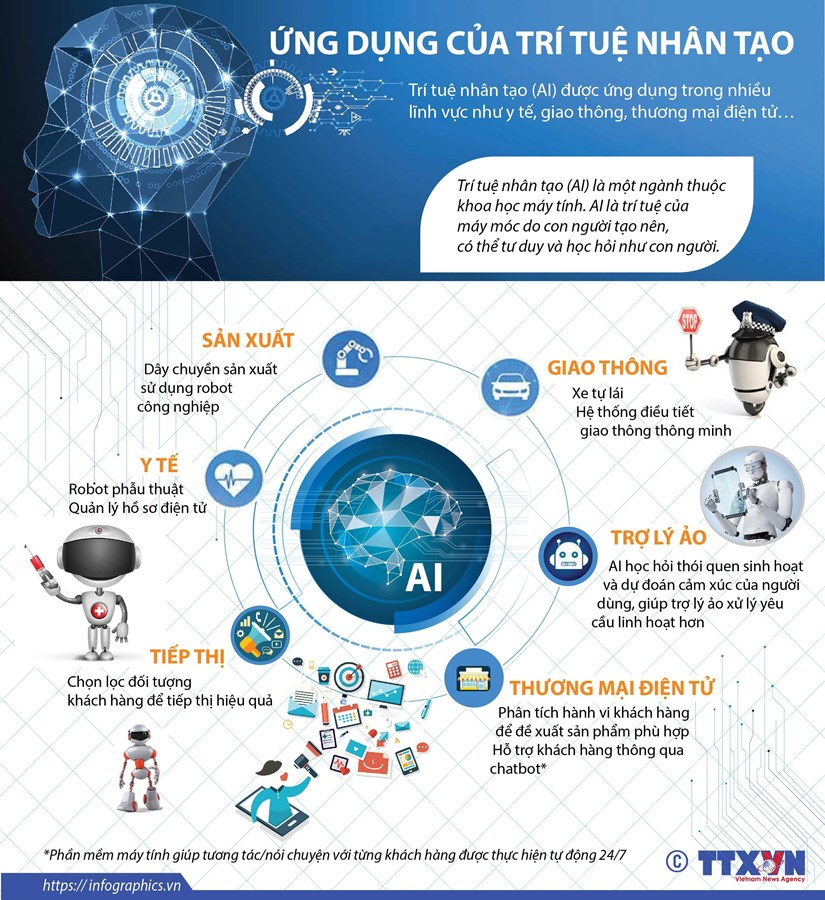
\includegraphics[width=0.6\textwidth]{image1.jpg}
	\centering
\end{figure}

Tại Việt Nam, AI đã và đang được ứng dụng mạnh mẽ trong nhiều lĩnh vực như y tế, giáo dục, nông nghiệp, giao thông, thương mại điện tử... Công nghệ AI cũng đã mang lại cho Việt Nam sự phát triển vượt bậc thời gian qua. Đặc biệt, vấn đề dữ liệu lớn, Việt Nam cần chia sẻ nhiều hơn cho cộng đồng, thậm chí là các quốc gia khác, bởi dữ liệu không nên chỉ nói trong phòng kín mà cần ở một mặt phẳng chung để lan tỏa và các quốc gia cùng chia sẻ.

Hệ thống giao thông thông minh (Intelligent Transport Systems – ITS) không phải là điều gì quá mới mẻ. Ý tưởng về hệ thống này đã được khởi xướng từ những năm 60, 70 của thế kỷ trước tại Mỹ và các nước Châu Âu. Đến nay, mô hình này đã được áp dụng thành công tại nhiều thành phố lớn trên thế giới.

Hệ thống giao thông thông minh là công nghệ được sử dụng để giải quyết các vấn đề của giao thông đường bộ, trong đó bao gồm việc xử lý tai nạn và ùn tắc giao thông. Về cơ bản, ITS sẽ sử dụng kết nối thông tin giữa hệ thống giao thông, phương tiện đang di chuyển và con người nhằm hình thành một mạng lưới, qua đó tối ưu việc vận hành và tham gia vào quá trình điều tiết giao thông.

Tại các nước châu Á, Hàn Quốc chính là quốc gia đi tiên phong trong việc ứng dụng công nghệ nhằm phát triển Hệ thống giao thông thông minh. Seoul (Hàn Quốc) được nhận định là thành phố có hệ thống giao thông thông minh tốt nhất thế giới.

Trong lĩnh vực giao thông vận tải tại TP Hồ Chí Minh, trí tuệ nhân tạo sẽ giúp thành phố có những phát triển vượt bậc trong công tác quản lý và điều hành hệ thống giao thông đô thị. Theo Sở Giao thông vận tải TP Hồ Chí Minh, có ba ứng dụng của AI trong việc hỗ trợ đối với lĩnh vực giao thông vận tải. Nếu như trước đây, việc đo đếm, phân tích lưu lượng, mật độ, vận tốc dòng giao thông tại các đô thị có đặc thù giao thông hỗn hợp với thành phần xe máy chiếm chủ yếu, được xem là không khả thi đối với các công cụ phân tích truyền thống như vòng từ, ống hơi hay cảm biến áp điện, thì giờ đây với sự phát triển của AI mà cụ thể là machine learning. Theo đó, hệ thống phân tích dữ liệu giao thông theo thời gian thực do Sở Giao thông vận tải TP Hồ Chí Minh đang triển khai thực hiện thông qua camera thu thập dữ liệu đạt đến mức độ chính xác khá cao, trên 90\% trong các điều kiện thời tiết, môi trường phức tạp và kỳ vọng tiếp tục tăng độ chính xác dữ liệu hành vi giao thông được thu thập ngày càng nhiều, phục vụ phân tích.

Với 775 camera giám sát giao thông được lắp đặt rộng khắp các tuyến đường giao thông trọng điểm, các nút giao thông phức tạp, hệ thống phân tích, giám sát giao thông tự động đang được Sở Giao thông vận tải TP Hồ Chí Minh triển khai nhằm kịp thời phát hiện, bố trí lực lượng điều tiết, bảo đảm trật tự an toàn giao thông cũng như cung cấp thông tin giao thông theo thời gian thực cho người dân thông qua Cổng thông tin giao thông trực tuyến và cách kênh thông tin khác.

Bên cạch việc phân tích phục vụ giám sát, điều hành giao thông trực tuyến, machine learning còn có thể hỗ trợ phân tích các hành vi vi phạm trật tự an toàn giao thông, như: vi phạm tốc độ, lấn làn, ngược chiều, lưu thông trên vỉa hè… hướng đến sử dụng hình ảnh thu thập từ camera để xử phạt “nguội” các phương tiện vi phạm.

Cùng sự hỗ trợ của khoa học công nghệ, từ AI, machine learning, công cụ mô phỏng, dự báo… hệ thống giao thông thông minh đang triển khai không chỉ phục vụ công tác quản lý, giám sát, đo đếm hằng ngày, giúp điều hành giao thông một cách hiệu quả hơn, mà còn có thể làm cơ sở để dự báo công tác đầu tư ngắn hạn cũng như làm quy hoạch dài hạn phát triển hệ thống giao thông đô thị.

Hiện tại tình trạng giao thông ở Việt Nam còn nhiều bất ổn do ý thức người dân chưa chấp hành tốt luật giao thông và một phần công tác quản lý giao thông chưa triệt để. Nếu công nghệ trí tuệ nhân tạo được áp dụng vào giao thông thì sẽ giúp công tác giao thông có được một lợi thế lớn. Chẳng hạn như sẽ giảm thiểu công việc của cảnh sát giao thông, do công an giao thông không thể giám sát được mọi nơi nên việc áp dụng trí tuệ nhân tạo sẽ dễ dàng bao quát mọi nơi với độ chính xác cao sẽ giúp phát hiện toàn bộ các phương tiện vi phạm luật giao thông. Tất cả các phương tiện vi phạm này sẽ bị ghi lại và bị xử phạt để cảnh cáo, từ đó sẽ hạn chế được nạn vi phạm giao thông tràn lan ở Việt Nam.

Từ đó, nhóm chúng em muốn làm một đề tài liên quan đến việc áp dụng trí tuệ nhân tạo vào lĩnh vực giao thông: Nhận diện các phương tiện đi ngược chiều trên các tuyến đường một chiều qua một camera lắp cố định (có thể bao quát được toàn bộ hai lòng đường, chẳng hạn camera lắp tại một vị trí trên cao chính giữa hai lòng đường Hoàng Quốc Việt) với mục tiêu là phát hiện toàn bộ các phương tiện đi ngược chiều, camera ghi lại và báo cáo cho hệ thống rồi tiến hành xử phạt.

\subsection{Lý do chọn đề tài}
Thứ nhất là việc áp dụng đột phát và nhanh cóng của deep learning vào năm 2012 đã đưa vào sự tồn tại các thuật toán và phương pháp phát hiện đối tượng hiện đại và chính xác cao như R-CNN, Fast-RCNN, Faster-RCNN, RetinaNet và nhanh hơn nhưng rất chính xác như SSD và YOLO. Sử dụng các phương pháp và thuật toán này, dựa trên deep learning và cũng dựa trên việc học máy đòi hỏi rất nhiều kiến thức về toán học và việc học sâu. Có hàng triệu chuyên gia lập trình và các nhà phát triển phần mềm muốn tích hợp và tạo ra các sản phẩm mới sử dụng object detection. Nhưng công nghệ này xa tầm tay của họ và phức tạp để hiểu và sử dụng thực tế của nó.

Thứ hai là hiện nay các thư viện mã nguồn mở về trí tuệ nhân tạo rất phổ biến và được công khai nên có thể dễ dàng áp dụng chúng để tự tạo ra những sản phẩm trí tuệ nhân tạo của chính mình, có thể kể đến các thư viện phổ biến như sau:

OpenCV (Open Computer Vision) là một thư viện mã nguồn mở hàng đầu cho xử lý về thị giác máy tính, machine learning, xử lý ảnh. OpenCV được viết bằng C/C++, vì vậy có tốc độ tính toán rất nhanh, có thể sử dụng với các ứng dụng liên quan đến thời gian thực. Opencv có rất nhiều ứng dụng như Nhận dạng ảnh, Xử lý hình ảnh, Phục hồi hình ảnh ...

CNN (Convolutional Neural Network – Mạng nơ-ron tích chập) là một trong những mô hình Deep Learning tiên tiến. Nó giúp cho chúng ta xây dựng được những hệ thống thông minh với độ chính xác cao như hiện nay. CNN được sử dụng nhiều trong các bài toán nhận dạng các object trong ảnh. Như hệ thống xử lý ảnh lớn như Facebook, Google hay Amazon đã đưa vào sản phẩm của mình những chức năng thông minh như nhận diện khuôn mặt người dùng, phát triển xe hơi tự lái hay drone giao hàng tự động.

YOLO (You only look once) là một mô hình CNN để detect object mà một ưu điểm nổi trội là nhanh, chính xác hơn nhiều so với những mô hình cũ. Với đầu vào là một bức ảnh, hệ thống sẽ khoanh vùng toàn bộ các vật thể xuất hiện trong bức ảnh đó. Hiện tại có 3 phiên bản là YOLOv1, YOLOv2, YOLOv3, phiên bản v3 cực kỳ nhanh và chính xác, tốc độ detect các object trong bức ảnh gần là ngay lập tức.

Thứ ba là trên thế giới tuy đã có những phần mềm ứng dụng trí tuệ nhân tạo vào giao thông nhưng có thể giá thành rất đắt đỏ và chưa phù hợp với đặc thù giao thông ở Việt Nam, cho nên nhóm em quyết định tạo ra một sản phẩm do chính tay người Việt làm, dựa trên đặc thù giao thông ở Việt Nam, để phục vụ người Việt.

Cuối cùng là mặc dù việc áp dụng trí tuệ nhân tạo vào đời sống ở trên thế giới đã rất phổ biến và đạt được nhiều thành công trên nhiều lĩnh vực nhưng ở Việt Nam còn rất hạn chế nên đây là một cơ hội để chúng em tạo ra những sản phẩm trí tuệ nhân tạo mang thương hiệu Việt Nam, giúp người dân nước mình được tiếp xúc nhiều hơn với các sản phẩm trí tuệ nhân tạo.

\subsection{Mục tiêu}
Thứ nhất là với mong muốn góp phần nâng cao ý thức của cộng đồng, giảm thiểu tai nạn giao thông, hướng tới phát triển thành phố thông minh, nhóm em áp dụng hệ thống trí tuệ nhân tạo vào giao thông để theo dõi, tự nhận biết các phương tiện giao thông đi ngược chiều và lưu dữ liệu phục vụ cho việc phạt nguội của cảnh sát giao thông. Từ đó sẽ giảm thiểu được công việc của cảnh sát giao thông và nâng cao độ chính xác trong việc bắt lỗi giao thông.

AI có thể phát hiện ra mẫu trong những dữ liệu phức tạp đến mức các chuyên gia cũng không nhận ra. Trong một số ứng dụng đặc thù như xử lý hình ảnh, AI đã bằng hoặc vượt khả năng của con người. Chính vì lẽ đó, khi được ứng dụng vào quá trình điều tiết giao thông, trí tuệ nhân tạo sẽ giúp giảm bớt nhân công nhưng lại tăng cường khả năng xử lý dữ liệu của hệ thống.

Thứ hai là trên thế giới tuy đã có những phần mềm đáp ứng được những mục đích trên nhưng có thể giá thành rất đắt đỏ và chưa phù hợp với đặc thù giao thông Việt Nam, cho nên nhóm em quyết định tạo ra một sản phẩm do chính tay người Việt làm, phù hợp với đặc thù giao thông ở Việt Nam, để phục vụ người Việt. Không những thế còn có thể kiếm được một khoản lợi nhuận lớn.

Thứ ba là tạo ra được một hệ thống làm việc nhanh chóng và chính xác, phân tích, xử lý dữ liệu gần như ngay lập tức, góp phần cải thiện hệ thống giao thông còn nhiều bất cập ở Việt Nam hiện nay.

Cuối cùng là tự tay tạo ra được một sản phẩm, nâng cao kiến thức về lập trình đặc biệt là trí tuệ nhân tạo, phục vụ công việc sau này.

Để đạt được mục tiêu trên, trước hết, nhóm em cần tìm hiểu các công nghệ và các thành tựu thế giới đã đạt được trong lĩnh vực trí tuệ nhân tạo cụ thể là các thành tựu trí tuệ nhân tạo đã đạt được trong giao thông vận tải, mà hiện nay ở Việt Nam vẫn chưa phổ biến

Để thực hiện được đề tài này, chúng em cần những công cụ sau: Một camera độ phân giải cao được lắp đặt tại trung tâm 2 làn đường, một hệ thống máy tính có cấu hình đủ mạnh để xử lý hình ảnh camera đưa về, sử dụng ngôn ngữ Python với các thư viện như OpenCV để nhận diện phần lòng đường, mô hình YOLO để detect các đối tượng trong hình ảnh (các phương tiện và chiều)

Tiếp đến, về lý thuyết nhóm em cần tìm hiểu quy trình xây dựng phần mềm các mô hình, các thư viện sẽ sử dụng

Sau khi tìm hiểu được các lý thuyết để xây dựng phần mềm thì nhóm em sẽ tiến hành khảo sát, phân tích tình hình giao thông thực tế ở Việt Nam

Sau khi khảo sát xong tìm hình giao thông Việt Nam nhóm em sẽ tiến hành xây dựng phần mềm

Và cuối cùng là tiến hành lắp đặt, thử nghiệm trong thực tế và đánh giá

Sau khi lắp đặt camera, cần một bước để hệ thống xác định ra 2 làn đường và chiều đi đúng của 2 làn với 2 cách sau: Cách 1 là làm thủ công, sau khi lắp sẽ quy định luôn cho hệ thống các tọa độ của hai làn đường và chiều đi đúng luôn. Cách 2 là để hệ thống tự động nhận diện, trước tiên là lòng đường, sử dụng thư viện OpenCV với các hàm như findContours() và convexHull() để xác định ra được hai làn đường, lưu tọa độ các đỉnh làn đường lại để dùng về sau. Tiếp đó là cần xác định chiều cho 2 làn đường vừa xác định, cần bỏ ra một ngày để hệ thống training, trong một ngày, với mỗi làn đường, hệ thống sẽ liên tục đếm các phương tiện di chuyển theo cả hai chiều, từ đó chiều nào có số lượng xe đi đông hơn sẽ là chiều đúng.

Tiếp đến, để xác định chiều đi của các phương tiện, trước tiên chúng em sẽ sử dụng mô hình YOLO để detect ra các phương tiện có trong bức ảnh, sau đó dựa vào các bức ảnh liên tục thì sẽ xác định được sự di chuyển của các phương tiện, từ đó xác định ra được chiều đi.

Sau khi xác định được chiều đi của phương tiện, hệ thống sẽ kiểm tra xem phương tiện này đang ở làn nào (làn đã được hệ thống xác định), và so sánh với chiều đi đúng của làn đó, nếu sai chiều thì hệ thống sẽ gửi thông tin bao gồm hình ảnh bằng chứng, thời gian, địa điểm vi phạm, biến số xe, loại phương tiện về để làm dữ liệu phục vụ cho việc phạt nguội của cảnh sát giao thông.

Kết quả đạt được: Một hệ thống làm việc khá nhanh và chính xác phân tích, xử lý dữ liệu gần như ngay lập tức, góp phần cải thiện hệ thống giao thông còn nhiều bất cập ở Việt Nam hiện nay.

\subsection{Cấu trúc đồ án}
\renewcommand{\labelenumi}{}
\renewcommand{\labelenumii}{\arabic{enumi}.\arabic{enumii}.}
\large
\begin{enumerate}
	\item \textbf{Chương 1: Giới thiệu}\\
	(Chương này sẽ nói lên sự phát triển vượt bậc và tầm quan trọng của trí tuệ nhân tạo, đặc biệt là trong lĩnh vực giao thông vận tải. Giải thích lý do chọn đề tài, nêu lên mục tiêu của đề tài và cuối cùng là trình bày cấu trúc của đồ án.)
	\begin{enumerate}
		\item Đặt vấn đề
		\item Lý do chọn đề tài 
		\item Mục tiêu đặt ra
	\end{enumerate}
	\item \textbf{Chương 2: Nghiên cứu tổng quan về đề tài}\\
	(Tìm hiểu về các sản phẩm, các thành tựu đã có thên thế giới về áp dụng trí tuệ nhân tạo vào lĩnh vực giao thông, tìm hiểu các thư viện sẽ sử dụng.)
	\begin{enumerate}
		\item Tìm hiểu về OpenCV
		\item Tìm hiểu về CNN và YOLO
		\item Các thành tựu trên thế giới về áp dụng trí tuệ nhân tạo trong giao thông
	\end{enumerate}
	\item \textbf{Chương 3: Phương pháp nghiên cứu}\\
	(Tiến hành lập trình phần mềm, các bước cài đặt và chuẩn bị. Nêu lên phương pháp, thuật toán nhận diện chiều phương tiện bằng YoLo.)
	\begin{enumerate}
		\item Cài đặt và chuẩn bị
		\item Nhận chiều phương tiện bằng YOLO
	\end{enumerate}
	\item \textbf{Chương 4: Thảo luận}\\
	(Dựa số liệu thực tế từ sản phẩm, đúc kết ra những cái đã làm được và những hạn chế chưa làm được. Đánh giá chất lượng sản phẩm.) 
	\begin{enumerate}
		\item Đánh giá số liệu
		\item Điểm mạnh
		\item Hạn chế
		\item Xem xét kết quả
	\end{enumerate}
	\item \textbf{Chương 5: Tổng kết}\\
	(Tổng kết đồ án tóm lược những cái đã làm, đánh giá tổng quan về các thành viên, mức độ hoàn thành công việc và chất lượng sản phẩm.)
\end{enumerate}

Cuối cùng với sự phát triển của AI và tình trạng giao thông Việt Nam hiện nay thì việc áp dụng trí tuệ nhân tạo vào là cần thiết, để triển khai trí tuệ nhân tạo vào việc điều hành, điều tiết hoạt động giao thông Việt Nam sẽ phải đối mặt với rất nhiều thách thức. Tuy vậy, nếu ứng dụng thành công trí tuệ nhân tạo, đây sẽ là lời giải cho bài toán giao thông vốn ngày càng hóc búa do sự phát triển quá nóng của các phương tiện tham gia giao thông tại Việt Nam cho nên nhóm em quyết định làm đề tài này để tăng độ chính xác trong việc bắt lỗi các vi phạm giao thông và giúp giải quyết vấn đề giao thông ở Việt Nam.

\section{Chương 2: Nghiên cứu tổng quan về đề tài}
\subsection{Tìm hiểu về OpenCV}
\subsection{Tìm hiểu về CNN và YOLO}
\subsection{Các thành tựu trên thế giới về áp dụng trí tuệ nhân tạo trong giao thông}
\section{Chương 3: Phương pháp nghiên cứu}
\subsection{Cài đặt và chuẩn bị}
\subsection{Nhận chiều phương tiện bằng YOLO}
\section{Chương 4: Thảo luận}
\subsection{Đánh giá số liệu}
\subsection{Điểm mạnh}
\subsection{Hạn chế}
\subsection{Xem xét kết quả}
\section{Chương 5: Tổng kết}
\section{Tài liệu tham khảo}
\renewcommand{\labelenumi}{[\arabic{enumi}]}
\begin{thebibliography}{9}
	\bibitem{opencv} BRADSKI, Gary; KAEHLER, Adrian, Learning OpenCV: Computer vision with the OpenCV library, O'Reilly Media, Inc, 2008.
	\bibitem{opencv2} BRADSKI, Gary; KAEHLER, Adrian, OpenCV. Dr. Dobb’s journal of software tools, 2000, 3.
	\bibitem{cnn} REN, Shaoqing, et al. Faster r-cnn: Towards real-time object detection with region proposal networks. In: Advances in neural information processing systems. 2015. p. 91-99.
	\bibitem{tvd} CIOLLI, Robert. Traffic violation detection, recording and evidence processing system. U.S. Patent No 8,134,693, 2012.
	\bibitem{link}https://nhandan.org.vn/khoahoc-congnghe/item/41678802-tp-ho-chi-minh-dua-tri-tue-nhan-tao-vao-y-te-giao-thong.html
	\bibitem{link}https://vietnamnet.vn/vn/cong-nghe/vien-thong/tri-tue-nhan-tao-loi-giai-cho-bai-toan-giao-thong-o-viet-nam-454016.html
\end{thebibliography}

\end{document}


